\section{Sesión 4}

\begin{cajita}
	A4: (De parejas) $\exists A\forall z\ni (z\in A\iff [z=x\vee z=y])$. 
\end{cajita}


\begin{teorema}(Construcción de conjuntos con dos elementos)
	$\exists ! A \forall z\ni (z\in A\iff [z=x\vee z=y])$. 
\end{teorema}

\begin{definicion}
	$w=\{x,y\}\iff [\forall z(z\in w\iff[z=x\vee z=y] )]$
\end{definicion}

\begin{teorema}(Varios)
	\begin{enumerate}
		\item 	$z\in \{x,y\}\iff [z=x\vee z=y]$.
		\item $\{x,y\}=\{u,v\}\implies [(x=u\wedge y=v)\vee (x=v\wedge y=u)]$.
	\end{enumerate}
\end{teorema}

\begin{teorema}
	$$\{x\}=\{x,x\}$$
	$$\{x,y,z\}=\{x,y\}\cup \{z\}$$
	$$\{w,x,y,z\}=\{w,x\}\cup \{y,z\}$$
\end{teorema}

\begin{teorema}
	$\{x\}=\{y\}\implies x=y$. 
\end{teorema}

\begin{definicion}(Pareja ordenada)
	\begin{enumerate}
		\item $(x,y)=\{\{x\},\{x,y\}\}$
		\item Si $\Delta \neq \square \implies (x,y)=\{\{x,\Delta\}, \{y,\square\}\}$
	\end{enumerate}
\end{definicion}

\begin{teorema}
	$(x,y)=(u,v)\implies [x=u\wedge y=v]$
\end{teorema}
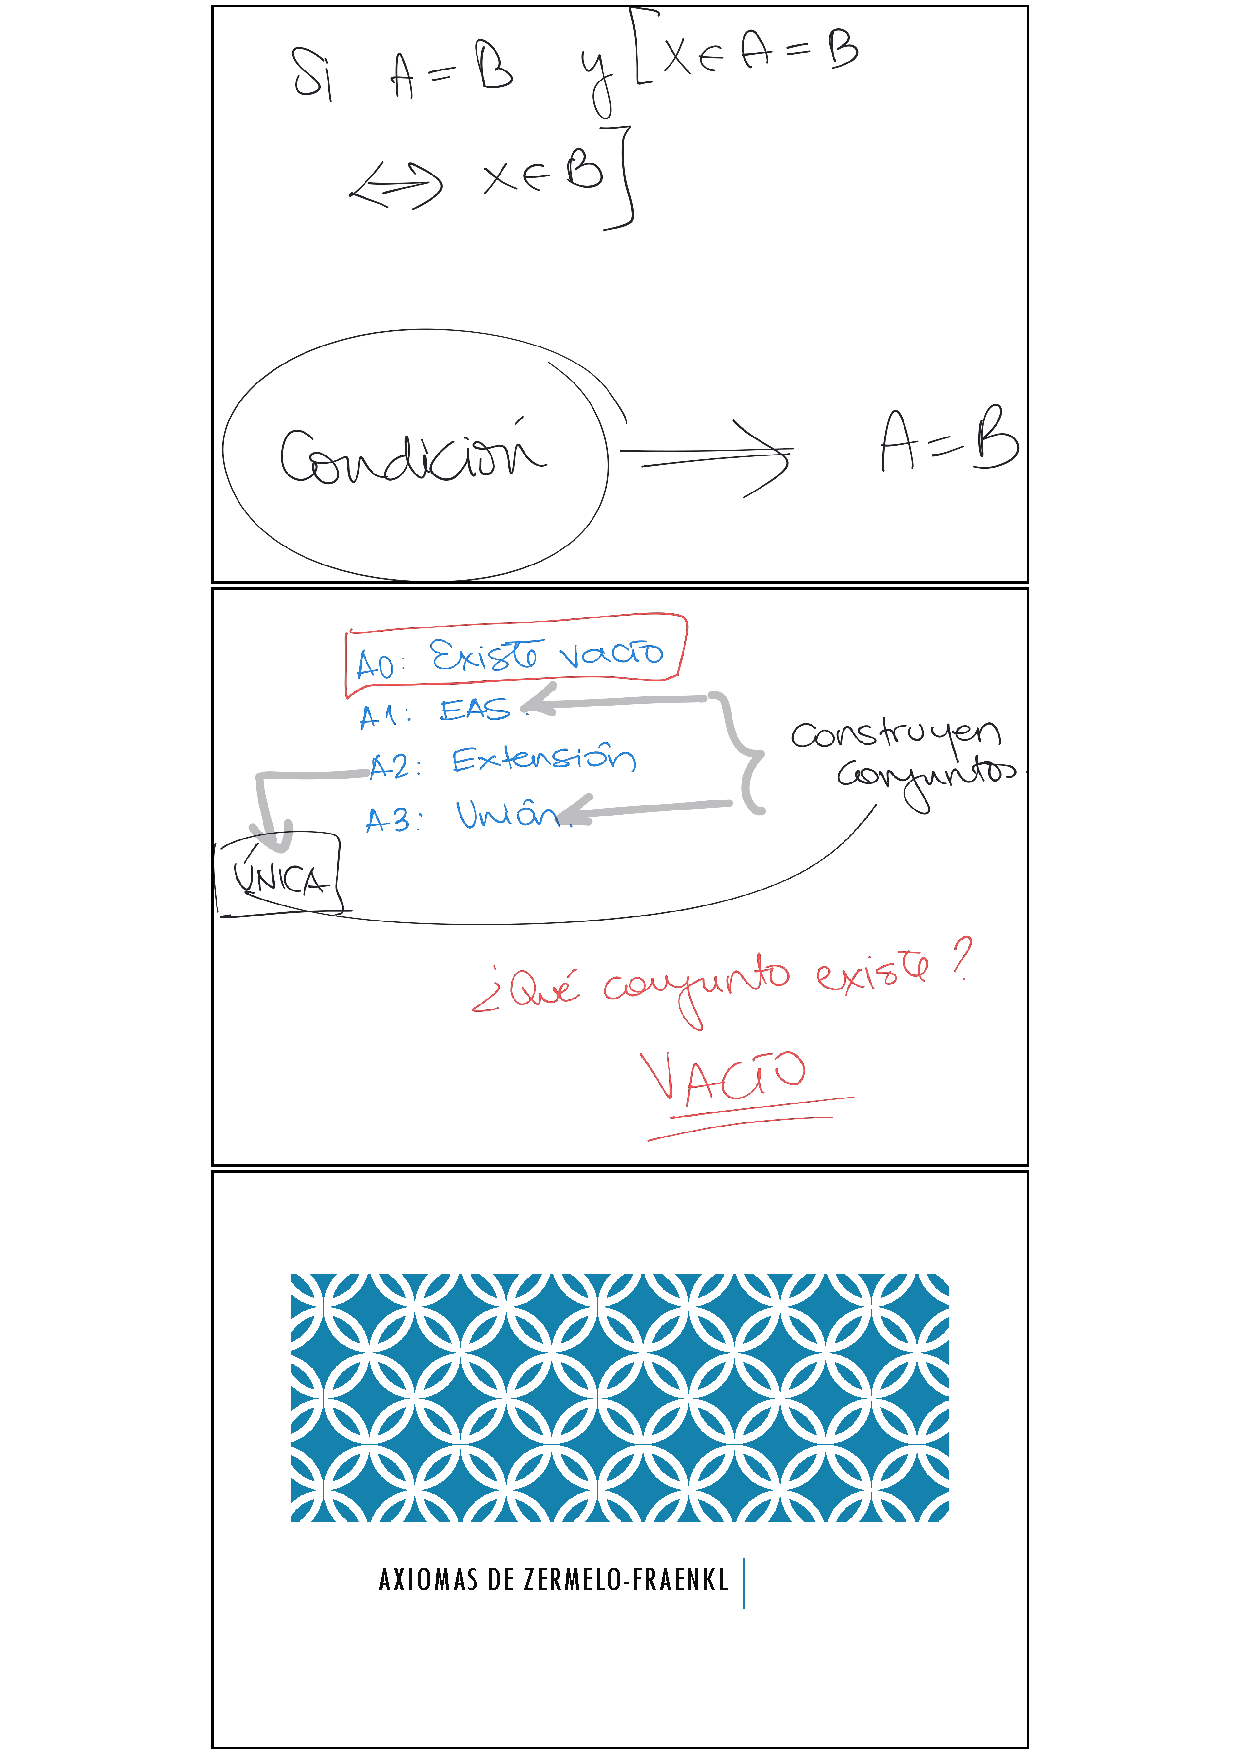
\includepdf[pages=-]{Apendices/s4.pdf}